\documentclass{beamer}
\usepackage[utf8]{inputenc}
\usepackage[graphicx]

\author[Sowmya Vajjala]{Instructor: Sowmya Vajjala}


\title[LING 120]{LING 120: \\ Language and Computers}
\subtitle{Semester: FALL '17}

\date{25 October 2017}

\institute{Iowa State University, USA}

%%%%%%%%%%%%%%%%%%%%%%%%%%%

\begin{document}

\begin{frame}\titlepage
\end{frame}
%http://psych.fullerton.edu/mbirnbaum/psych101/Eliza.htm
\begin{frame}
\frametitle{Outline}
\begin{enumerate}
\item LING 410X advertisement 
\item Question from last class
\item A text classification algorithm: Naive Bayes
\item Chatting with Eliza: Exercise
\end{enumerate}
\end{frame}

\begin{frame}
\frametitle{LING 410X: Language as Data}
\begin{itemize}
\item Introductory course on data science - but specific to working with text
\item Intended audience: people from different LAS backgrounds, and with no pre-reqs.
\item Content: Methods of working with text data (collecting, pre-processing, storing, mining knowledge, doing text classification, visualizing text etc.
\item Means: R programming language and associated libraries.
\item First taught in Spring 2017. To know about syllabus, assignments, and projects - you can talk to me. 
\end{itemize}
\end{frame}

\begin{frame}
\frametitle{Question from last class}
\begin{enumerate}
\item Let us say you are working on classifying webpages as "appropriate" and "inappropriate" for children and you developed two classifiers. 
\item Now let us say you have a test set that has 500 texts labeled "appropriate", 250 texts labeled "inappropriate".
\item Here are the confusion matrices for Classifiers A and B: \\
\begin{table}[h]
\begin{center}
\begin{tabular}{r}
  \begin{tabular}{|l|r|r|}
    \hline
    (A) pred. $\rightarrow$&\textbf{App.}&\textbf{Inapp.}\\
    \hline
    \textbf{App.}&490&10\\ \hline
    \textbf{Inapp.}&200&50\\ \hline
    \end{tabular}
  \begin{tabular}{|l|r|r|}
    \hline
    (B) pred. $\rightarrow$&\textbf{App.}&\textbf{Inapp.}\\
    \hline
    \textbf{App.}&400&100\\ \hline
    \textbf{Inapp.}&50&200\\ \hline
    \end{tabular}
\end{tabular}
\caption{Confusion matrices for two scenarios}
\end{center}
\end{table}
\item What is the classification accuracy for A and B respectively?
\item According to you, which one is doing better? A or B? Why? 
\end{enumerate}
\end{frame}

\begin{frame}
\frametitle{Follow up}
Which one is better:
\begin{table}[h]
\begin{center}
\begin{tabular}{r}
  \begin{tabular}{|l|r|r|}
    \hline
    (A) pred. $\rightarrow$&\textbf{App.}&\textbf{Inapp.}\\
    \hline
    \textbf{App.}&500&0\\ \hline
    \textbf{Inapp.}&200&50\\ \hline
    \end{tabular}
  \begin{tabular}{|l|r|r|}
    \hline
    (B) pred. $\rightarrow$&\textbf{App.}&\textbf{Inapp.}\\
    \hline
    \textbf{App.}&300&200\\ \hline
    \textbf{Inapp.}&20&230\\ \hline
    \end{tabular}
\end{tabular}
\caption{Confusion matrices for two scenarios}
\end{center}
\end{table}
Note: Also wrote replies to comments posted on 23rd Oct forum explaining these. Check that out. 
\end{frame}

\begin{frame}
\frametitle{How do we evaluate?}
\begin{itemize}
\item In general, overall accuracy is a good measure. However, it may not be the best one if you need one category to be more accurate than the other. 
\item In this case: Tagging appropriate ones as inappropriate ones is bad, but tolerable. But tagging inappropriate ones as appropriate is dangerous, because children will end up having access to inappropriate content. 
\end{itemize}
\end{frame}

\begin{frame}
\frametitle{Steps in Text classification?}
\begin{itemize}
\item We need a collection of example texts with known categories (Training data)
\item We need to extract "features" we want the machine to learn from these (feature extraction)
\item \textbf{We should take these extracted features and give them to a "learning algorithm" (training/learning phase)}
\item Evaluate if the "learned" classifier is doing well by "testing" it with a few more examples with known categories (test data, evaluation)
\item If you are happy, start using in some real-world application!!
\end{itemize}
\end{frame}

\begin{frame}
\frametitle{Naive Bayes Classifier}
\begin{itemize}
\item Simplest, easy to understand method to do classification
\item Primarily relies on probability and bayes theorem
\item Although it is not the best algorithm around, it is commonly used to set a baseline whenever you see a new text classification problem.
\end{itemize}
\end{frame}

\begin{frame}
\frametitle{}
\begin{center}
\Large Probability Primer
\end{center}
\end{frame}

\begin{frame}
\frametitle{What is probability?}
\begin{itemize}
\item In our class, there are about 20 people. 
\item If I have to randomly (and unbiasedly) pick one person to ask a question now, what is the probability that it is Emily? \pause Answer: 1/20
\item What is the probability that it will be Emily or Ethan? \pause Answer: 1/20 + 1/20 = 2/20 (it may turn out I can pick Emily again too).
\item What is the probability that I pick either a Freshman or an International Student? \pause
\\ Formula: P(Freshmen) + P(Intl. student) - P(Freshmen who are Intl. students).
\end{itemize}
\end{frame}

\begin{frame}
\frametitle{What is probability? - Examples}
\begin{itemize}
\item Look at this age distribution for 10 students: 
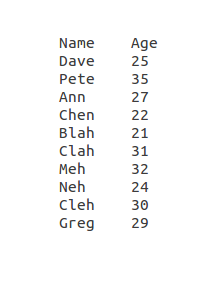
\includegraphics[width=0.3\textwidth]{prob1.png}
\item If I randomly pick one person, what is the probability that this person is below 30 years of age? \pause Ans: 6/10
\item If I randomly pick one person, what is the probability that it is Dave? what is the probability that this is not Dave? \pause Ans: 1/10 and 9/10.
\end{itemize}
\end{frame}

\begin{frame}
\frametitle{Conditional probability}
\begin{itemize}
\item Conditional probability is the probability of one event happening, when we know some other event has happened before.
\item If one of my events is seeing 2 when I roll a die (E1), the other event is seeing an even number (E2), then, P(E1$|$E2) is: 1/3. Why?? \pause
\item What is P(E1)? \pause 1/6
\item What is P(E2)? \pause 3/6 i.e., 1/2
\item What is P(E1, given E2) \pause E2 has three possibilities (2,4,6). So, probability of getting 2 is 1/3.
\end{itemize}
\end{frame}

\begin{frame}
\frametitle{Joint probability}
\begin{itemize}
\item Probability that two events occur together. Represented as P(A,B) and is the same as P(B,A)
\item So what is the difference between joint and conditional probability? \pause
\item Useful example: \url{https://goo.gl/9MVM78} \pause
\item Additional information: 
\begin{itemize}
\item Conditional probability is not commutative P(A$|$B) != P(B$|$A)
\item P(A,B) = P(A$|$B)*P(B) =  P(B$|$A)*P(A)
\end{itemize}
\end{itemize}
\end{frame}

\begin{frame}
\frametitle{Bayes Theorem}
\begin{itemize}
\item $P(A | B) =\frac{P(B |A)* P(A)} {P(B)}$ - this is the theorem.
\item Example when applied to Spam classification: 
\begin{enumerate}
\item P(Spam$|$Email) = $\frac{P(Email|Spam)*P(Spam)}{P(Email)}$
\item P(Ham$|$Email) = $\frac{P(Email|Ham)*P(Ham)}{P(Email)}$
\item Each time we see a new email, we calculate these two probabilities. If the first one is higher, we classify the email as spam. Else, as ham!
\end{enumerate}
\item P(Email) and P(Spam) are probabilities of seeing the Email and Probability of a spam email in your training data.
\item How do we get P(Spam)? \pause
\item How do we get P(Email)? \pause Do we even need it? \pause
\item What is the difference between P(Spam$|$Email) and P(Email $|$ Spam)? \pause
\end{itemize}
Reading recommendation: \url{http://www.ling.upenn.edu/courses/cogs501/Bayes1.html}
\end{frame}

\begin{frame}
\frametitle{How do we combine all evidence?}
%PUT FIGURE FROM LAST WEEk
\begin{itemize}
\item We are operationalizing an email as a bunch of words.
\item So ohow should we calculate P(Email$|$Spam) and P(Email$|$Ham)? \pause
\item Product of individual word probabilities! 
\\ P(Email$|$Spam) = P(Spam) * $\Pi_f$P(f$|$Spam) 
\\ P(Email$|$Ham) = P(Ham) * $\Pi_f$P(f$|$Ham)
\\ Where f stands for "feature". In our example, we took words. But other features are: "is it all upper case", "is there large amounts of money mentioned" etc.  
\end{itemize}
\end{frame}

\begin{frame}
\frametitle{For further study}
\begin{itemize}
\item We spoke briefly about others like - looking for nearest neighbors, creating a linear separator between classes, neural networks etc. 
\item There are 100s more. 
\item For more mathematical orientation on these, you should take a Machine Learning course
\item For more practical applications, you should take courses on areas where machine learning is used to solve specific problems - such as natural language processing and computer vision.
\item ISU offers a lot of these courses!
\item Something to get started: \url{https://web.stanford.edu/~jurafsky/slp3/} (Chapter 6)
\end{itemize}
\end{frame}

\begin{frame}
\frametitle{Preview to next topic: Attendance exercise}
Post on Canvas.
\begin{itemize}
\item go to: \url{http://psych.fullerton.edu/mbirnbaum/psych101/Eliza.htm}
\item Chat with Eliza for sometime and write your comments on the interaction addressing the below questions:
\item Is it doing a good job of chatting? What is happening - how do you think is it able to understand what you say?
\item Does it fail? In what cases?
\end{itemize}
\end{frame}

\end{document}


